\documentclass{scrartcl}
\title{\rmfamily Software Engineering -- Blatt 10}
\author{Rasmus Diederichsen \and Felix Breuninger\and 
   \texttt{\{rdiederichse, fbreunin\}@uos.de}
}
\date{\today}
\usepackage[ngerman]{babel}
\usepackage[space]{grffile} % for spaces in includegraphics fnames
\usepackage{marvosym, microtype, textcomp, xifthen, multirow, booktabs, dingbat,
   titlesec, enumitem, fullpage, tikz, IEEEtrantools, array, amsmath, listings,
   colortbl,
amssymb, graphicx, subcaption, lmodern,pgfplots}
\usepackage[pdftitle={Software Engineering -- Blatt 10}, 
   pdfauthor={Rasmus Diederichsen, Felix Breuninger}, 
   hyperfootnotes=true,
   colorlinks,
   bookmarksnumbered = true,
   linkcolor = lightgray,
   plainpages = false,
citecolor = lightgray]{hyperref}
\usepackage[utf8]{inputenc}
\usepackage[T1]{fontenc}
\usepackage[all]{hypcap}
\titleformat{\section}[hang]{\bf}{Aufgabe 10.\arabic{section}:}{1em}{}[]
\titleformat{\subsection}[hang]{\bf}{\hspace{1em}\alph{subsection})}{1em}{}[]

\lstset{
   frame=single,
   basicstyle=\ttfamily\small,
   frameround=tttt,
   backgroundcolor=\color{lightgray!10},
   keywordstyle=\color{teal}\textbf,
   stringstyle=\itshape,
   showstringspaces=false,
   language=[gnu] make,
   morecomment=[n]{$(}{)},
   commentstyle=\color{blue},
   title=\lstname
}
\usetikzlibrary{shapes,positioning,calc,decorations.text,graphs,arrows.meta}
\begin{document}

\fontfamily{ptm}\selectfont
\maketitle

\section{Evolutionäre / inkrementelle Modelle}

\subsection{Inkrementelle Modelle}

Der inkrementelle Entwicklungsprozess ist durch folgende Aspekte gekennzeichnet:
\begin{itemize}
   \item Software im Allgemeinen zunächst als Kernprodukt abgeliefert
   \item Nach und nach werden Features hinzugefügt
   \item Jedes Feature durchläuft einen kompletten Entwichklungszyklus (z.B. wie
      im Wasserfallmodell)
   \item Frühere Releases sind abgespeckte Versionen der späteren.
   \item Inkremente werden anhand der Benutzung des vorherigen Releases durch
      den Kunden durchgeplant unt entwickelt.
\end{itemize}

\newcolumntype{V}{>{\columncolor{green!10}\flushleft\arraybackslash}p{.4\textwidth}}
\newcolumntype{N}{>{\columncolor{red!10}\flushleft\arraybackslash}p{.4\textwidth}}
\begin{center}
   \begin{tabular}{VN}
      \toprule
      \textbf{Vorteile} & \textbf{Nachteile} \\ 
      \midrule
       Schneller Weg zur fertigen Kernfunktionalität & Unklar, wann es ``fertig'' ist \\
       Es werden keine Releases weggeworfen, Qualitätsarbeit in jeder Iteraion  & Inkremente v. A. nach User-Feedback $\rightarrow$ schwer planbar \\
       Entwicklung kann bei Einhaltung on Restriktionen dennoch stets fertiges
       Produkt liefern (Ressourcenknappheit, Deadlines, Warten auf Technologien,
       etc.) & \\
       Beliebige Erweiterbarkeit (potenziell langlebig) & \\
       Kurze Iterationen machen Fehler weniger teuer & \\
       Nachträgliche Ergänzungen einfach einzubauen & \\
   \end{tabular}
\end{center}

\begin{figure}
   {\centering      
   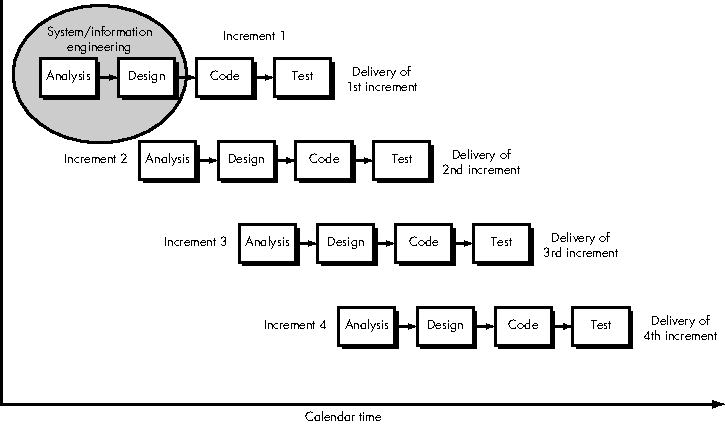
\includegraphics[width=\textwidth]{incremental_pressman.pdf}
   \caption{Iteratives Vorgehensmodell}
   \label{iter}}
\end{figure}

\subsection{Evolutionäre Modelle}

Das evolutionäre Vorgehen ist charakterisiert durch
\begin{itemize}
   \item Anforderungen, Pläne, Designs, Aufwandsschätzungen etc. entwickeln sich
      über die Zeit
   \item Entwicklung verläuft iterativ, indem die einzelnen Phasen nach
      Anpassung der Spezifikationen wiederholt werden
   \item In jeder Iteration werden die Bestandteile der Phasen (s.o.) verfeinert 
   \item im Spiralmodell schreitet die Entwicklung spiralförmig fort, indem
      aufbauend auf dem Produkt der vorherigen Iteration immer alle Phasen neu
      durchlaufen werden.
   \item Anders als beim rein inkrementellen Vorgehen durchlaufen nicht einzelne
      Features den Entwicklungsprozess und werden ``angetackert'', sondern die
      Gesamtsofware wird überarbeitet.
\end{itemize}

\begin{center}
   \begin{tabular}{VN}
      \toprule
      \textbf{Vorteile} & \textbf{Nachteile} \\ 
      \midrule
      Hohe Anpassbarkeit an Kundenvorstellungen & Schwer planbar, da Anforderungen nicht zu Anfang bekannt\\
      Schneller Prototyp & Versionen werden verworfen \\
      Anforderungen müssen nicht alle zu Beginn bekannt sein & Häufige
      Änderungen sind schwer zu überblicken und können zu schlechterem Code
      führen \\
      Sämtliche Projektdokumente werden verbessert, alles ist konsistent & \\
      Prozess hat kein Ende, kann gesamte Lebensdauer abdecken & Kein klares
      Ende \\
      Zu keinem Zeitpunkt im Lebenszyklus werden Aspekte vernachlässigt. & \\
   \end{tabular}
\end{center}

\begin{figure}
   {\centering      
      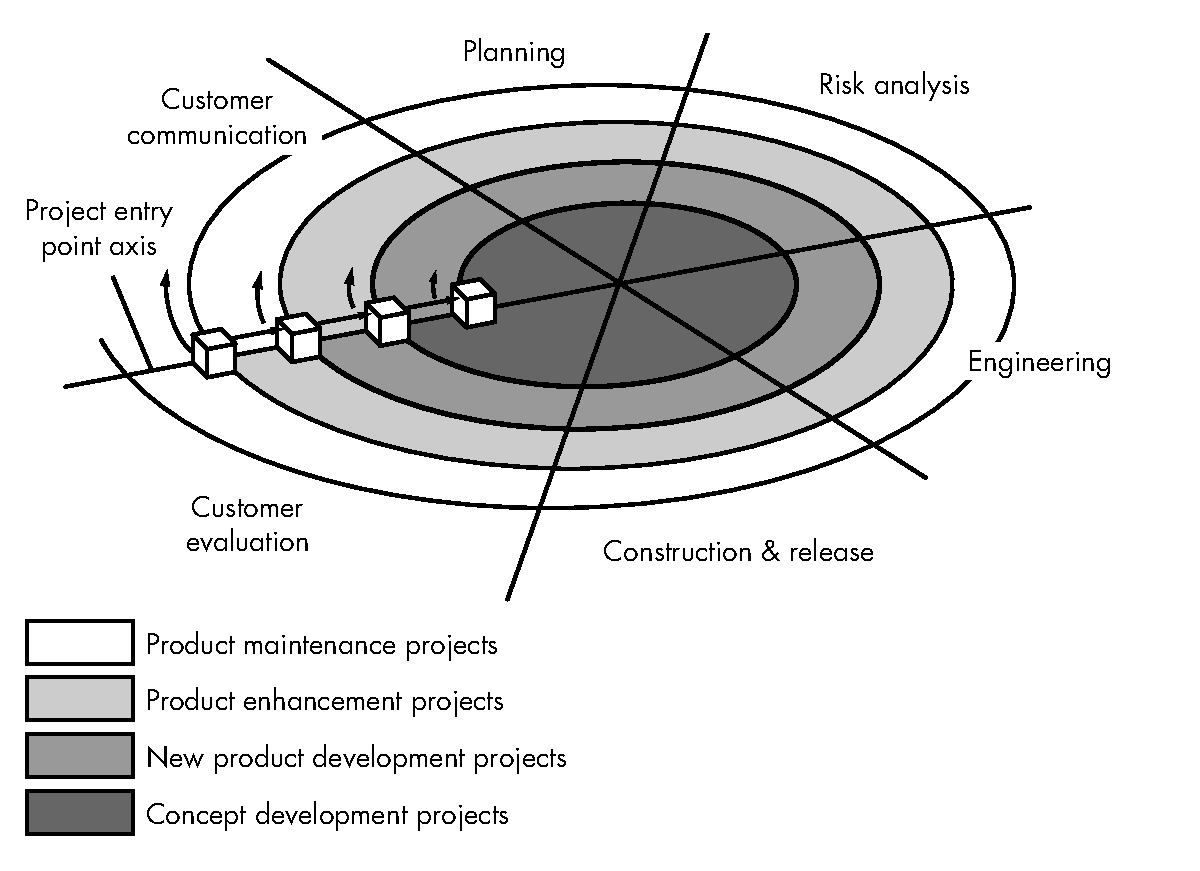
\includegraphics[width=\textwidth]{evol_pressman.pdf}
   \caption{Spiralmodell; Evolutionäres Vorgehen mit definierten Task Sets}
   \label{evo}}
\end{figure}

\vspace{\baselineskip}
\noindent\textbf{Quellen}:
\begin{enumerate}
   \item \emph{Pressman, R.: Software engineering: a practitioner’s approach, 5th ed.}
   \item \emph{Larman, C.: Agile and Iterative Development: A Manage's Guide}
\end{enumerate}
\section{Vorgehensmodelle}
\begin{enumerate}
   \item Da die Anforderungen bekannt sind und ein strikter Zeitplan möglich
      ist, bietes sich ein lineares Vorgehen wie Wasserfall oder V-Modell an.
      Es ist nicht erforderlich, möglichst schnell etwas präsentieren zu können,
      also muss man nich agil vorgehen.
   \item Rapides Prototyping erlaubt, das Problem notdürftig zu hotfixen, der
      Fix kann dann verbesert werden.
   \item Evolutionär vorzugehen, würde es erlauben, die zwangsläufig
      auftretenden Änderungen miteinzubeziehen.
   \item Das V-Modell expliziert die Notwendigkeit und Zuständigkeit
      verschiedener Tests
   \item Seems legit. Code-and-Fix wäre hier ausreichend, da Dr. Blair kein
      Softwareingenieur ist und nur flott etwas demonstrieren muss. Die Software
      wird weder wirklich benötigt, noch wird sie länger in Betrieb sein.
\end{enumerate}

\section{Scrum}

\section{Kanban}


\end{document}
